\section{Introduction}
In the context of the personal project course given at ULiège. I decided to develop a smart freezer. This idea emerges due do a personal experience. Every year my family and I reorganize the home's freezers. I was a bit shocked when I saw the quantity of products that were in the freezers and for which I was not aware. This is a problem that anyone can potentially face one day. \\

The main problem of forgotten products is they cannot stay indefinitely to a freezer due to they physical properties. For instance after some time a meat staying for a long time into a freezer will not have a good taste. As results, some products were thrown to the rubbish. We could avoid to throw to the rubbish products if we are aware of the existence of that products. The solution of that problem would be an application or a tool that gives the possibility to manage the content of your freezers and more. It is the direction that I took for my personal project.

\subsection{Explanation of the project itself}
The aim of the project is to provide a freezer system manager that gives to a user using this system some information about his products. This system also keep an history of a user's products. Moreover, the main purpose of that system manger is to give the possibility for a third person to develop its own application and use the freezer system manager inside of it. It is personal choice and I took this option because I appreciate open-source applications and I would like to bring my personal contribution to the open-world. \\

The information that the system manager need to take into account are:
\begin{enumerate}
\item The user that uses the system manager.
\item A unique token linked to this user. This token is necessary to interact with the system.
\item A password and an identifier (email address) linked to that user. These two information are essential to obtain the token.
\item The language that the user uses. This information is not used in the scope of the project but it is a useful information to store if we want to extend the project later.
\item The freezers linked to this user. This information is fundamental because we need to locate a product.
\item The products linked to a user. A product is defined by several features: 
\begin{enumerate}
\item A product name.
\item A description of the product given by the user.
\item A quantity in terms of people (e.g: a meal for 2 people).
\item A product type (e.g; vegetable, soup,...).
\item A date of input and output
\item A period during which a product may remain inside a freezer.
\item An identification inside a freezer (e.g: the product number 2 in box 3 of the freezer number 1).
\end{enumerate}
\end{enumerate}

These information must to be stored in a database with some other data. The architecture of this database and data stored are explained in details in the section made for that purpose.\\

As explained above, the aim of the system manager is to give the possibility for a user using the system to find what he wants, where a product is located,... The freezer system manager cannot be used directly because we want to give access to the freezer system manager for third applications but we do not want that these third applications have the possibility to modify or destroy the system manager architecture.\\

To get around this problem the interaction with the freezer system manager is done through a REST API. REST API is commonly used by companies who want to give access to their data or a piece of their data to third applications without giving direct access to their databases. The main advantages of a REST API is that it is a client-server which means that the server evolves independently of the client and it is stateless. Moreover, A REST API allows to develop an application on any terminal. It is possible to develop an application for raspberry Pi or for a smartphone. Since REST API is stateless and we want to identify a user We need a method to go around this problem. It is the aim of the token. The token allows to detect uniquely a user if it is correctly generated. A schema given \autoref{fig:archi} shows where the REST API is set. \\
\begin{figure}[H]
\centering
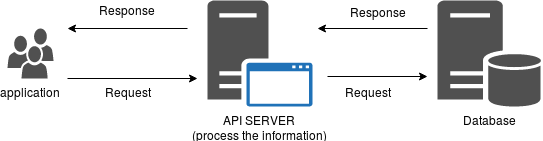
\includegraphics[scale=0.5]{./images/archi.png}
\caption{REST API interaction}
\label{fig:archi}
\end{figure}

The token generated is static but in general a token has an expiration date. I do not go into that direction because it becomes complex to manage such token with an API.\\

With a user token and the REST API, a user has the possibility to find what he wants. He can add new products, he can edit existing products, he can see what are the products he has in a specific freezer. He also has the possibility to see the historic of a freezer. Moreover, the API can make suggestions for the user according to his previous consumptions and depending on what his freezers contain.\\

To give the possibility to third people to understand how the API works. I made a documentation for that purpose with examples that show how it works and what are the results obtained. \\

Finally, to demonstrate the utilization of a third application with the REST API. I built a website that only uses the API to manage the freezers of a specific user.\\

%expliquer brièvment les différentes sections qui vont etre abordée dans ce qui suit et l'architecture du code

\section{Content storing}
\subsection{Database model discussion}
To store the different information about a user and the data related to his freezers a database is required. There exists several types of databases and it is not easy to make a choice that will not have bad impacts on the future if the choice made at the beginning was not good. The choice made is a relational database. this choice is motivated by several things. First of all, the problem is known and links to establish between data are known. Moreover, data would not change on the long-term which means that the architecture of the database would not change a lot and the quantity of information to store will never be huge. In addition, data to store is essentially texts and numbers, thus no need to have a database that can manage video streams like noSQL database. Finally,
the relational database architecture is probably the architecture which is the easiest one to be ported into another database architecture like \textit{Cassandra} or \textit{MongoDB} or anything else.\\

The relational database management system chosen is MySQL since it is an open-source software which is commonly use. Moreover, it does not require too much work to set it up.

\subsection{Relational database structure}
The information that the database need to store will be explained in detailed.\\

First of all, we need to store some information about a user such as an email which is unique and a password that allows the user to establish a connection with the internal website. This website is an integral part of the freezer system manager and gives additional information about the user such as the token linked to the user account. This token is mandatory to have access to the freezer system manager API and it is generated uniquely. It is also used to identify a user. \\

A user has also two additional information which are the language and learning fields. The language field is used to specify the language used by the user as explained earlier. It can be interesting for third applications to have some knowledge about the user. The learning field is used to save some parameters that could be useful for learning algorithm. For this project I do no use it because I did not have enough time to find and test some of these algorithms. To summarize a user is defined through 5 fields which are a token, a password, an email, a language, and a learning.\\

After defined a user, we need to defined the other objects that will be stored and linked to a user.\\

The database contains several types of products. These types of products can only be added by the administrator of the system to avoid inconsistencies that users can bring by adding weird product types or by defining several time the same type. We need to keep in mind that some users just want to break the system instead of using it. A product type is described by a unique identification number automatically generated by the database, the name of the product type in English and in french. The identification number allows to locate and retrieve the information of a specific product type. If we want to extend the number of languages we can add news columns in the database without affecting the architecture or using a translation tool to translate the existing into the desired language. Since translation tools are very powerful. The second proposition seems to be more adequate. To summarize a product type is defined through 3 fields which are an type identification, an English type name, and a French type name.\\

To store user's products we need to formally define how a freezer is described. A freezer is described with three fields which are a unique identification number, the number of boxes that the freezer has and the name given to this freezer. The identification number is used to locate and retrieve a specific freezer. It is automatically generated by the database. To summarize a freezer is defined through 3 fields which are the freezer identification, the number of boxes that the freezer contains, and a freezer name.\\

A freezer product from a user contains several fields. First of all, a unique identifier given by the system itself. A date of input, this date must be anterior to the date of its entrance in the freezer. In other words it is impossible to encode product with a date that refers to a place in the future. A date of output, by default this field is set to null. When this field is not null it means that the product is not any more in the freezer. The date of output must be greater or equal to the date of input. A product also contains a period field which is used to define the period in months for which the product should be in the freezer. Thus, third applications can display products that overcome this period. The quantity is also a piece of information of a product. It gives  the quantity in terms of person for whom the product can be used. Finally, a product also has two additional fields to allow a user to locate more easily a product. These two additional fields are the box number which give the box for a specific freezer and the product identifier which allows to locate the product in this box. This identifier is unique for the specific box.\\

A product also receives a description . The product description contains three different fields which are the description identifier, the product name and a free description of the product. This description can be a structured description or a simple text. \\

Now that we know what the database will contain and the links that exist between the different elements, we can establish the entity-relationship model that will make it easier to visualize our database. This is explained in details in the following section.

\subsection{Entity-relationship model}
The \autoref{fig:reldb} shows the entity-relationship model of the freezer database. As we can see on this schema the relations \textit{list\_freezer} and \textit{product\_to\_type} are not mandatory since the information that they linked can be retrieved from the rest of the database. These two relations have been inserted into the database for a simplicity since these information are often asked. Knowing that it is interesting for the backup part. \\

\begin{figure}[H]
\centering
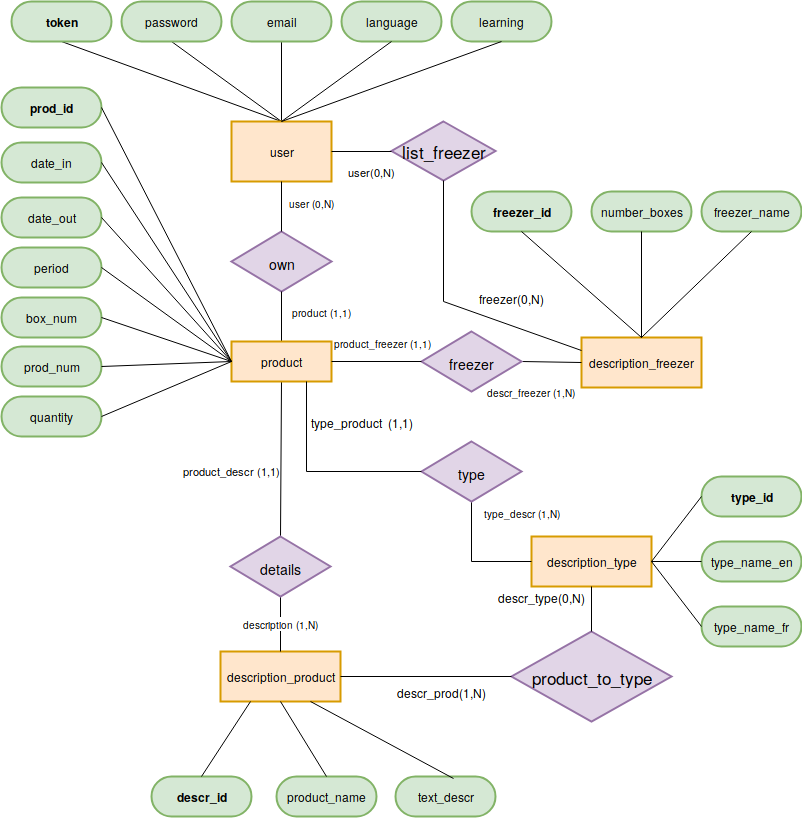
\includegraphics[scale=0.5]{./images/reldb.png}
\caption{entity-relationship model of the database}
\label{fig:reldb}
\end{figure}

\subsection{Relational model}
From the entity-relationship we can go into the relational format which allow to have a representation for integrating the database into a relational database management system.
\begin{enumerate}
\item User(\underline{\textbf{token}}, password, \underline{email}, language, learning)
\item Description\_type(\underline{\textbf{type\_id}}, type\_name\_en , type\_name\_fr)
\item Description\_product(\underline{\textbf{descr\_id}}, product\_name, text\_descr)
\item Description\_freezer(\underline{\textbf{freezer\_id}}, number\_boxes, freezer\_name)
\item Product\_to\_type(\textbf{\#descr\_id, \#type\_id})
\item List\_freezers(\textbf{\#freezer\_id, \#token})
\item Product(\underline{\textbf{prod\_id}}, \#token, \#descr\_id, \#freezer\_id, \#type\_id, date\_in, date\_out, period, box\_num, prod\_num, quantity)
\end{enumerate}

The database is encoded in \textit{MySQL} language. The engine used is \textit{InnoDB} with utf8mb4\_unicode\_ci as collation. The choice of this engine has been done because is the default engine and manage ACID transactions and foreign keys. The \autoref{fig:sqldb} depicts the \textit{MySQL} implemented and the types associated to each variable. The choices made for the length size of variables are personal choices. But the length size can be changed with no difficulties if the need arose. The encoding chosen allows to be flexible as much as possible.

\begin{figure}[H]
\centering
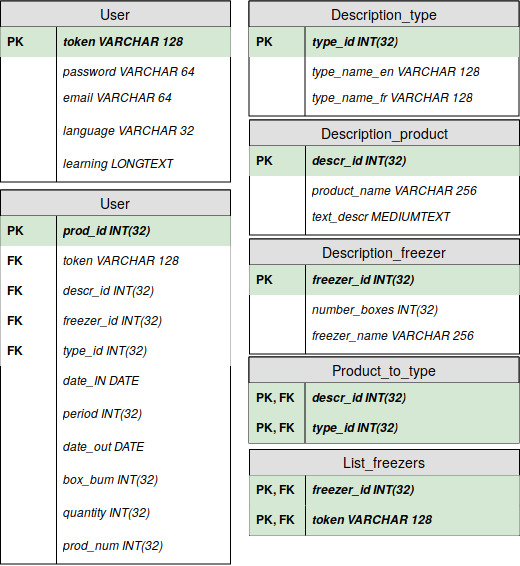
\includegraphics[scale=0.5]{./images/sqldb.jpg}
\caption{slq tables of the database}
\label{fig:sqldb}
\end{figure}

As discussed above the architecture of the database allows to skip some tables to backup like Product\_to\_type and List\_freezers. These two table can be reconstruct with the others tables. Thus it is not mandatory to backups these ones.\\

To use the database we need to fill it with some data. This filling part has been done manually. The reason of that is to represent something that has a sense and can represent a lambda user. Moreover, I made this choice because initially I wanted to develop some preference learning algorithm and in this optic fill a database with random objects has no sense. 

\section{Internal website}
After the startup of the database, we need to give the possibility for new users to create an account to have access to the freezer API and manage your freezers. Without an account a user cannot do anything. It is the reason why an application to create and manage a user account is needed.\\

The type of application chosen to manage these things is a website. This choice has been made because we can have a tool that is running on a browser and it avoids the potential conflicts from an OS to another. The languages used for the website development are html/css and Javascript for the front-end and PHP for the back-end. PHP is a server-side language which is commonly used when we develop a website and it allows to interact with the MySQL database. \\

The internal website is divided into three distinct parts. The first one concerns the account creation, the second concerns a user panel that can be accessed when an account is created, and the last section is dedicated to the admin panel. This panel is only dedicated to the administrator of the freezer application. \\

The recommanded protections for a website are not configured. To secure a website some files such as \textit{.htaccess} or \textit{php.ini} need to be correctly set in accordance with the server. Moreover, the redirection pages are not configured and/or personalized but for a production website it is required.

\subsection{Account creation}
To use the API a user need to create an account with an e-mail address and a password. A webpage (\autoref{fig:register}) is built to achieve this goal( \textit{website/register.php}). To have a the password encrypted, a PHP function called \textit{crypt()} is used with a salt. By default crypt uses the DES algorithm. This algorithm was the most widely used algorithm during many years. Nowadays this algorithm is not secure to crypt data but in the case of the project is the algorithm chosen.\\
If the objective is to put in production the project. It is recommended to change the password encryption to use another type of encryption like SHA 512 or another secure encryption algorithm.\\

When the account has been created it is linked to a token. This token is generated on the server side with the PHP function \textit{random\_bytes} which is recommended to generate string of cryptographic random bytes that are suitable for cryptographic use. The length  specified for the generation is 32 bytes. Thus, the number of possibilities is $(2^8)^{32} = 2^{256}$. After that, the random sequence generated is transformed into a hexadecimal string to be more readable by a novice user.\\
\begin{figure}[H]
\centering
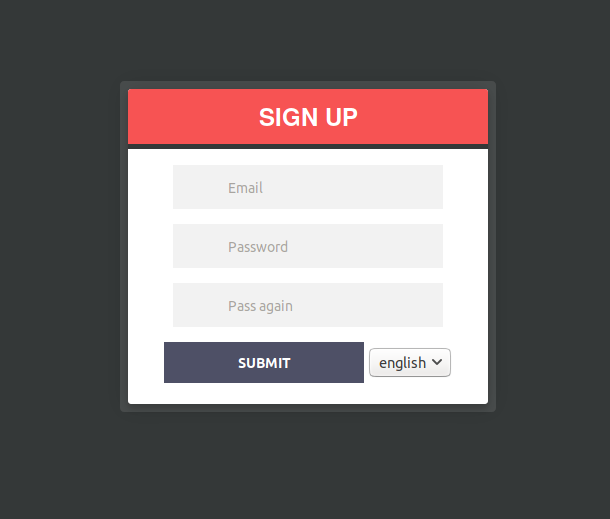
\includegraphics[scale=0.4]{./images/register.png}
\caption{register page}
\label{fig:register}
\end{figure}

When the account is created a user can use the API to build its own software and manage his freezers with the help of The API and the token linked to its account or use an existing application that uses the API. The third part applications should only asked your token and anything else.\\

\subsection{User panel}
When a user possesses an account. He has the possibility to access to a user panel of the freezer system manager with the \textit{website/login.php} page (\autoref{fig:login}). If the information given are correct, he will be redirected to the user panel page \textit{website/user/user\_interface.php}.
\begin{figure}[H]
\centering
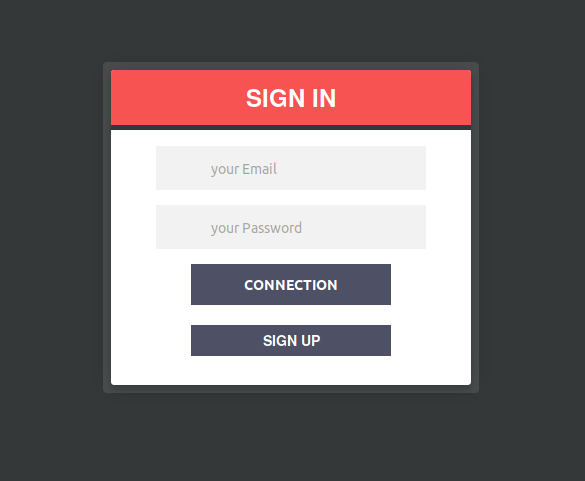
\includegraphics[scale=0.4]{./images/login.png}
\caption{Login page}
\label{fig:login}
\end{figure}

This user panel is used to give to the user more information about its account. i.e: the email address, the token linked to the account, the possibility to change the password and the language. For the scope of the project the user panel is not developed more than that but for production project it should be the case. We could add some features to manage our freezers, etc.

\begin{figure}[H]
\centering
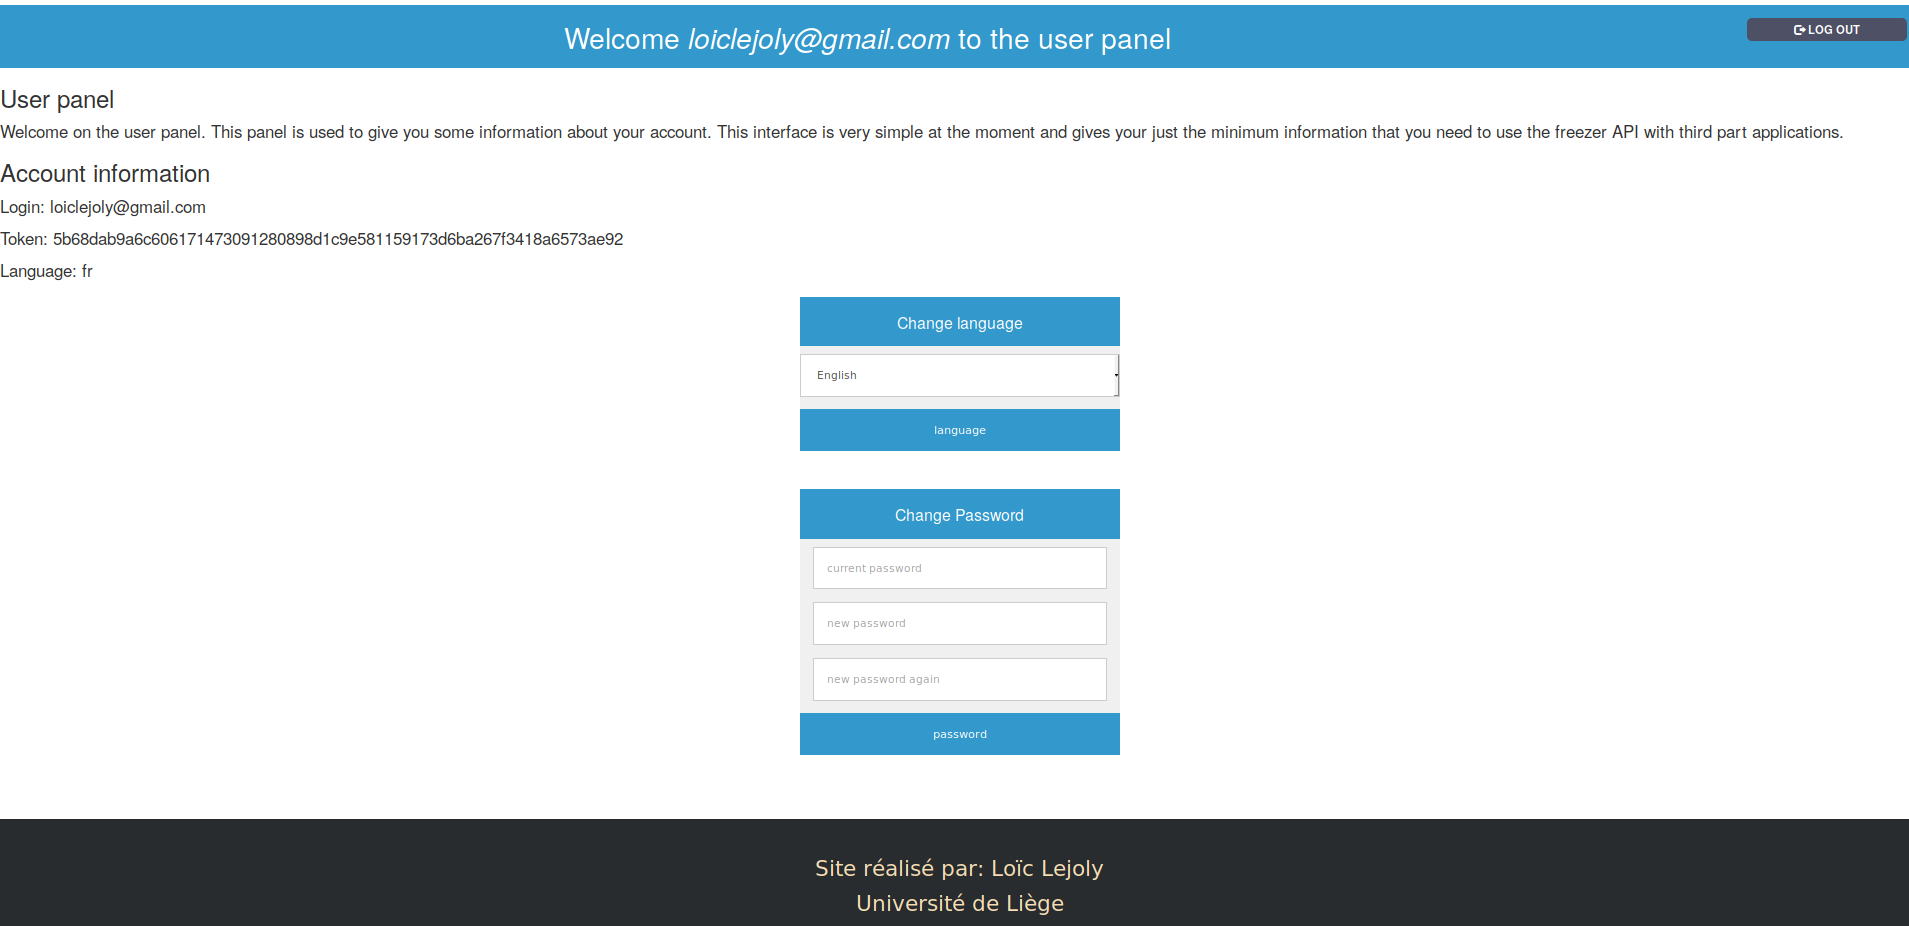
\includegraphics[scale=0.25]{./images/userPanel.png}
\caption{User panel}
\label{fig:login}
\end{figure}
\subsection{Admin panel}
It is interesting for a system administrator to have access to an admin panel. In general, an admin panel is used to manage a system and more specifically the database linked to it. It allows to have a global view of the system. Analyse information about a specific user. Manage the system by applying some updates. Compute some statistics and more. In the scope of the project, I built a really simple panel that only allows to list and add a new product type. I would have liked to develop it in details but I did not have enough time to do that and it potentially be too much work for the scope this course.\\

The \autoref{fig:adminLogin} shows the admin login page. As we can see this page is really simple. To have the possibility to connect to the admin panel you need to give a identifier (admin) and a password (root). These two informations are hard-coded in the \textit{website/admin/login.php}. For a practical case this approach is not recommanded. Instead of encoding these informations inside a php file it is recommanded to store it in the \textit{.htaccess} file or inside a configuration file like \textit{config.ini}. This allows to separate the code from the configuration and sensitive information.
\begin{figure}[H]
\centering
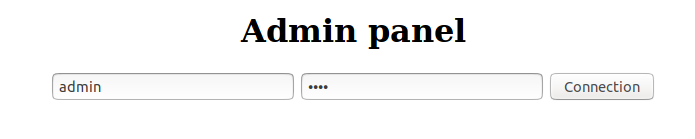
\includegraphics[scale=0.4]{./images/adminLogin.png}
\caption{admin login page}
\label{fig:adminLogin}
\end{figure}

When the identifier and the password given are correct. You will be redirected to the admin panel \autoref{fig:adminPanel}. As we discussed above, the admin panel is very simple. You have the possibility to display and hide the different product types, you can also add a new product type.
\begin{figure}[H]
\centering
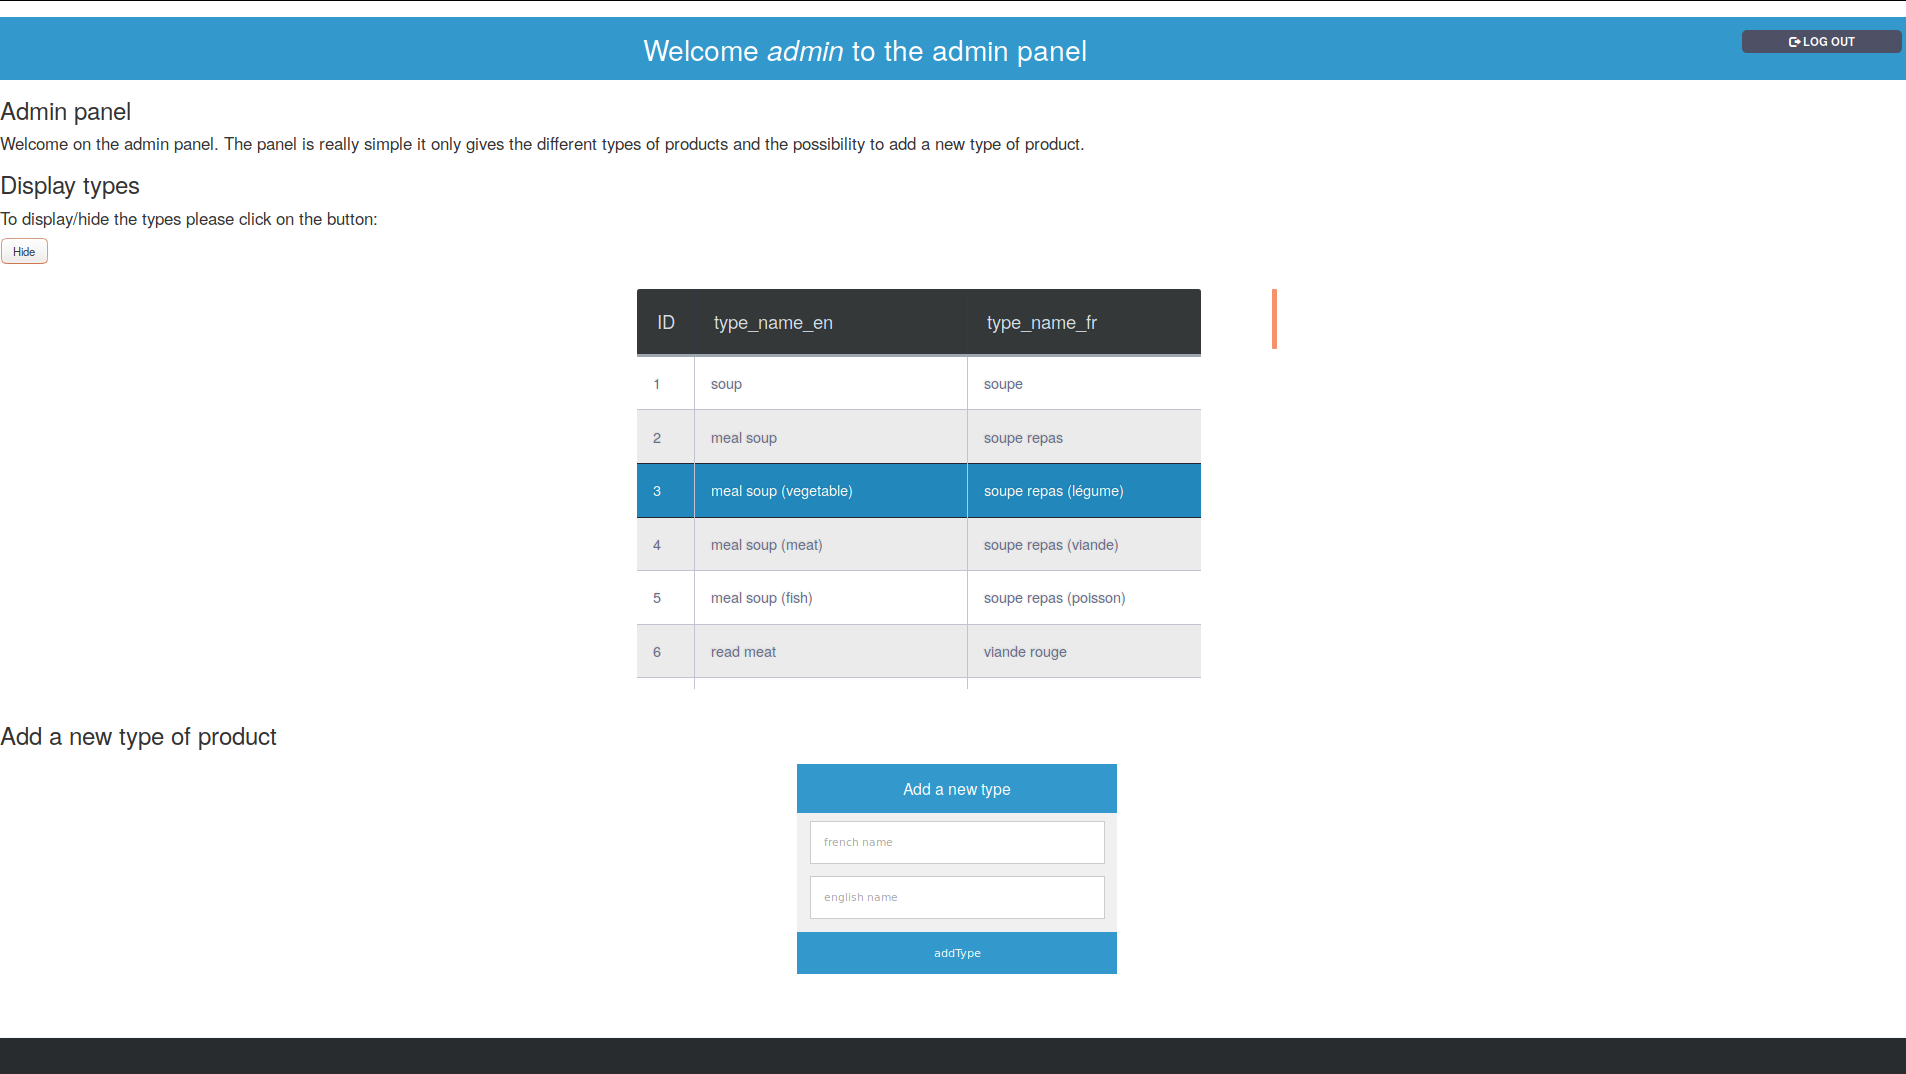
\includegraphics[scale=0.25]{./images/adminPanel.png}
\caption{admin login page}
\label{fig:adminPanel}
\end{figure}

\section{API REST}
A REST API is built on a server that establishes a communication between the database and the the client. REST API is useful for several reasons. The first reason is that it is a client-server that means the server evolves independently of the client. Moreover, with a REST API you can develop applications without worrying about changes in queries since they are the same on any terminal. Finally, new functionalities can be added easily since the REST API is based on URI. We Just need to specify a new URI and specify what the request need to achieve.\\

The REST API server implemented in the project scope cannot be really called a RESTful server because all specifications asked to be certified as REST are not fulfilled. A layered system and cacheability are not implemented because it was too complex to set up and I would have spent a lot of time to set up these parts.\\

Since the REST API needs to work with bowers which specify in request headers the field \textit{Origin} for some type of requests \textit{POST}, the REST API needs to use cross-origin resource sharing (CORS). The CORS allows the REST API server to accept the ajax requests which are forbidden due to the same-origin security policy.\\

%% parler de l'intauration d'un limiter par IP pour éviter des requetes pérpétuelle d'un utilisateur
%% le serveru flask tourne en single thread pour la version 0.12.2
%%unicorn pour prod
\subsection{Folder architecture}
The REST API follows the folder architecture given below. The folder \textit{tests} is used to implement the different unit tests done on the server. The others files defined at the root of the REST\_api folders are used to build the server itself.

\dirtree{%
.1 REST\_api.
.2 tests .
.3 tests.py .
.2 mysqlRequests.py .
.2 queryDB.py .
.2 responseMessage.py .
.2 sever.py .
.2 utils.py .
.2 validatorDB.py .
}

\begin{enumerate}
\item \textit{mysqlResquests.py}: This module defines the major part of requests done by the API. It only contains variables that are PURE sql strings. It is simpler to maintain sql requests with a separate file where sql requests are defined instead of looking in the core of the server.
\item \textit{queryDB.py}: This module implements a class \textit{QueryDB} that is used to send SQL requests and retrieve data of them.
\item \textit{responseMessage.py}: This module defines the detailed response messages that are send with an error status code. It only contains English strings. With this method it is possible to change the language of the messages sent simply by overriding these variables with the appropriate text.
\item \textit{server.py}: This module is the server core it implements the server. It is the module to run to set the server up.
\item \textit{utils.py}: This module implements some functions used by other modules. 
\item \textit{validatorDB.py}: This module implements a class \textit{ValidatorDB}. This class is used to validate parameters that will be sent with the mysql request. It avoids to bring inconsistencies in the database due to incorrectly done user requests.
\end{enumerate}
\subsection{Sever}
As you can see with the folder description above, the server is developed in python. I made this choice because I wanted to discover the possibilities offered by this language but others languages are also perfectly fit to achieve that such as Java, PHP, Javascripts,...\\

A micro-framework is used to develop the Python server with Python language. This framework is Flask and it is build an Werkzeug and Jinja 2. The version of Flask used to develop this project is 0.12.2. The stable version of the micro-framework just comes up (26th 2018) with a number of changes. \\

To interact with the mysql database I used the module MysqlDB \footnote{\url{https://github.com/PyMySQL/mysqlclient-python}}. This module is not the best known nor the most used. Nevertheless, this module allows to write sql requests in a pure sql fashion. I chose this module instead of others well known modules based on a Object Relational Mapper (ORM) such as sqlachemy for two reasons. The first one is that an ORM like sqlalchemy makes abstractions of the sql part. It can be an advantage in terms of optimizations, to manage cursors,... The drawback of ORM is that you cannot necessarily understand what is behind this module. The second reason is that the set up of ORM is no so easy to do correctly. It seems understandable since the ORM makes abstraction of sql part. Thus, I made the choice to take the MysqlDB instead of sqlachemy module. Nevertheless, for a production application, it is recommended to use an ORM because these tools are optimized to achieved requests, They give the possibility to change database type without changing all requests in the code. Moreover, the application can be maintained by people not necessarily mastering the SQL language.
\subsection{functionalities implemented}
Several functionalities have been implemented. For each request done by a user, parameters sent with the requests are parsed to avoid SQL injection. Moreover, type parameters are also checked. A first check is automatically  done by the flask micro-framework by checking the format of the URI.

For instance the URI format specified in the the server follows:
$$ @app.route("/myRequest/<int:identifier>")$$

If a user gives a string \textit{myIdentifier} as parameter flask automatically detects that the URI format is not correct and simply returns a status code 404 because the route with this URI format does not exist.\\

If all parameters have a correct type the server will check the consistencies of the data sent with the request. If data is consistent the sever can interact with the database otherwise an error status code is returned. An object with a detailed explanation is also returned with an error status code. This JSON object has two fields \textit{details and status}. The \textit{status} field contains the error status code sent and \textit{details} field contains a text that explains the reason of that status code.
 
\subsubsection{check\_token}
This request implements a single method which is \textit{GET} method. It gives the possibility to check the validity of a given token. If this one is correct a response with the status code 200 is sent. Otherwise, an error status code is sent with a JSON object as explained before.\\

The prototype of this request is the following:

$$<domainUrl>/check\_token/<token>$$

Parameters:
\begin{enumerate}
\item <domailUrl>: The url of the server API. In the case of the project the server is run on the \textit{localhost:5000}
\item <token>: A user's token that corresponds to an existing account.
\end{enumerate}

\subsubsection{types}
This request implements a single method which is \textit{GET} method. It gives the possible types of products that can be encoded into the database. To obtain these types you need to give an existing token. If this token is correct a JSON object containing the different types of products is sent and the status code of the response is 200. Otherwise, an error status code is sent with a JSON object as explained before.\\

The prototype of this request is the following:

$$<domainUrl>/types/<token>$$

Parameters:
\begin{enumerate}
\item <domailUrl>: The url of the server API. In the case of the project the server is run on the \textit{localhost:5000}
\item <token>: A user's token that corresponds to an existing account.
\end{enumerate}

The architecture of the JSON file returned is the following:
\begin{lstlisting}
[
    {
        "type_id": 1,
        "type_name_en": "soup",
        "type_name_fr": "soupe"
    },
    {
        "type_id": 2,
        "type_name_en": "meal soup",
        "type_name_fr": "soupe repas"
    },
    ...
]
\end{lstlisting}

Explanation of the  JSON object:
\begin{enumerate}
\item \textit{type\_id}: An `integer` that represents the id of the product's type
\item \textit{type\_name\_en}: The type name in English
\item \textit{type\_name\_fr}: The type name in French
\end{enumerate}

Note that it is not possible for a user to add a product type. It is the desired behaviour since we do not want a user with the possibility to add random product types or define several times the same product type. This functionality only given to the admin of the system. This functionality is implemented for the admin website.

\subsubsection{Freezer}
This request implements a four methods which are \textit{GET},\textit{POST}, \textit{PUT}, and \textit{DELETE}. These methods are used to manage the user's freezers and they share a common prototype:

$$<domainUrl>/freezer/<token>$$

Parameters:
\begin{enumerate}
\item <domailUrl>: The url of the server API. In the case of the project the server is run on the \textit{localhost:5000}
\item <token>: A user's token that corresponds to an existing account.
\end{enumerate}

\paragraph{GET method:} This method is used to retrieve information about the different freezers that a user possesses. This information is a list that contains all user's freezers and each freezer is described by three elements which are the identifier, the name, and the number of boxes that the freezer contains. If this token is correct a JSON object containing the information about the user's freezers is sent and the status code of the response is 200. Otherwise, an error status code is sent with a JSON object as explained before.\\

The architecture of the JSON format is:
\begin{lstlisting}
[
    {
        "freezer_id": 1,
        "freezer_name": "freezer 1",
        "number_boxes": 4
    },
    {
        "freezer_id": 3,
        "freezer_name": "freezer cave",
        "number_boxes": 6
    },
    ...
]
\end{lstlisting}

\paragraph{POST method:} This method is used to add a new freezer for a specific user. To add a new freezer data sent must follow a certain data type. The content-type sent must be a \textit{application/json}. If another content-type is sent, the request does not work and the status code 415 is returned in addition with two fields \textit{details and status} described earlier. If the  content-type is correct the JSON sent must respect the architecture given below. If the user token, the  content-type, and the JSON object sent are correct the response status code 200 is received. Otherwise, an error status code is sent with a JSON object as explained before.\\

The architecture of the JSON object to send must be:
\begin{lstlisting}
{
    "num_boxes": "4",
    "name": "my_name"
}
\end{lstlisting}

Explanation of the  JSON object:
\begin{enumerate}
\item \textit{num\_boxes}: An `integer` that represent the number of boxes.
\item \textit{name}: An `string` that represents the new name given to the freezer.
\end{enumerate}

\paragraph{PUT method:} This method is used to update an existing freezer which belongs to a specific user. To update a specific freezer data sent must follow a certain data type. The content-type sent must be a \textit{application/json}. If another content-type is sent, the request does not work and the status code 415 is returned in addition with two fields \textit{details and status} described earlier. If the  content-type is correct the JSON sent must respect the architecture given below. If the user token, the  content-type, and the JSON object sent are correct the response status code 200 is received. Otherwise, an error status code is sent with a JSON object as explained before.\\

The architecture of the JSON object to send must be:
\begin{lstlisting}
{
    "freezer_id": the id of an exisitng freezer,
    "num_boxes": "4",
    "name": "my_name"
}
\end{lstlisting}

Explanation of the  JSON object:
\begin{enumerate}
\item \textit{freezer\_id}: An `integer` that represents the id of an existing freezer that belongs to the user with the token given.
\item \textit{num\_boxes}: An `integer` that represents the number of boxes. Can be leaved empty if we do not want to update the number of boxes.
\item \textit{name}: A `string` that represents the new name given to the freezer. Can be leaved empty if we do not want to update the freezer name.
\end{enumerate}

\paragraph{DELETE method:} This method is used to delete an existing freezer which belongs to a specific user. To remove a specific freezer data sent must follows a certain data type.  The content-type sent must be a \textit{application/json}. If another content-type is sent, the request does not work and the status code 415 is returned in addition with two fields \textit{details and status} described earlier. If the content-type is correct the JSON sent must respect the architecture given below. If the user token, the content-type, and the JSON object sent are correct, the response status code 200 is received. Otherwise, an error status is sent with a JSON object as explained before.\\

The architecture of the JSON object to send must be:
\begin{lstlisting}
{
    "freezer_id": the id of an exisitng freezer
}
\end{lstlisting}

Explanation of the  JSON object:
\begin{enumerate}
\item \textit{freezer\_id}: An `integer` that represents the id of an existing freezer to delete.
\end{enumerate}

\subsubsection{freezer\_next\_id}
This request implements a single method which is \textit{GET} method. It gives the possibility to obtain the next available identifiers of all boxes of a specific freezer. These available identifiers represent the number that will be attributed for a new product of the concerned freezer box. If the request is correctly done a JSON object containing the next available box identifiers for a specific freezer and the status code of the response is 200. Otherwise, an error status code is sent with a JSON object as explained before.\\

The prototype of this request is the following:

$$<domainUrl>/freezer\_next\_id/<freezer\_id>/<token>$$

Parameters:
\begin{enumerate}
\item <domailUrl>: The url of the server API. In the case of the project the server is run on the \textit{localhost:5000}
\item <freezer\_id>: An integer that represents the id of an existing freezer that belongs to the user with the token given.
\item <token>: A user's token that corresponds to an existing account.
\end{enumerate}

The architecture of the JSON file returned is the following:
\begin{lstlisting}
{
  "1": 8, 
  "2": 3, 
  "3": 4, 
  "4": 3
}
\end{lstlisting}
Where for instance, "1" represents the box number and 8 the next available id for the product in the box 1.

\subsubsection{get\_product}
This request implements a single method which is \textit{GET}. It give the possibility to retrieve products of a specific user by specifying some parameters to the request. As for other get requests If the request is correctly done a JSON object containing information and the status code of the response is 200 are returned. Otherwise, an error status code is sent with a JSON object as explained before.\\

The prototype of this request is the following:

$$<domainUrl>/get\_product/<param>/<freezer\_id>/<token>$$

Parameters:
\begin{enumerate}
\item <domailUrl>: The url of the server API. In the case of the project the server is run on the \textit{localhost:5000}
\item <params>: A string that define the parameter that we want three parameters are possible:
\begin{enumerate}
\item \textit{all}: Selects all products.
\item \textit{inside}: Selects only products that are inside freezers.
\item \textit{outside}: Selects only products that are outside freezers.
\end{enumerate}
\item <freezer\_id>: An integer that represents the id of an existing freezer that belongs to the user with the token given. If we want to select all freezers that belongs to a user the id 0 must be specified.
\item <token>: A user's token that corresponds to an existing account.
\end{enumerate}

\begin{lstlisting}
[
  {
    "box_num": 1, 
    "date_formatted_in": "2016-12-31", 
    "date_formatted_out": "2017-03-02", 
    "descr_id": 2, 
    "freezer_id": 1, 
    "freezer_name": "frigo 1", 
    "period": 6, 
    "prod_num": 2, 
    "product_name": "glace vanille", 
    "quantity": 1, 
    "text_descr": "glace maison au aromatis\u00e9e \u00e0 la vanille", 
    "type_id": 24
  },
  {
    "box_num": 1, 
    "date_formatted_in": "2017-12-26", 
    "date_formatted_out": null, 
    "descr_id": 4, 
    "freezer_id": 1, 
    "freezer_name": "frigo 1", 
    "period": 6, 
    "prod_num": 4, 
    "product_name": "Soupe de No\u00ebl", 
    "quantity": 4, 
    "text_descr": "Soupe \u00e0 base de tomate, brocolli et poisson", 
    "type_id": 1
  },
  ...
  ] 
\end{lstlisting}
The JSON object returned is a list of element with the architecture shown above.
Explanation of the different elements
\begin{enumerate}
\item \textit{box\_num}: Represents the freezer box where the product is stored.
\item \textit{date\_formatted\_in}: Represents the input date of the product in the freezer. The format of the date is YYYY-MM-DD.
\item \textit{date\_formatted\_out}: Represents the output date of the product in the freezer. The format of the date is YYYY-MM-DD. If there is no output the value is simply null.
\item \textit{descr\_id}: The identifier of the product description.
\item \textit{freezer\_id}: The identifier of the freezer.
\item \textit{freezer\_name}; The freezer name.
\item \textit{period}: The period in months for which the product can stay in the freezer.
\item \textit{prod\_num}: The identifier of the product inside the freezer box.
\item \textit{product\_name}: The name of the product.
\item \textit{text\_descr}: The description of the product.
\item \textit{type\_id}: The type identifier of the product.
\end{enumerate}

\subsubsection{add\_product}
This request implements a single method which is \textit{POST}. It give the possibility to add a new product into a existing freezer for a specific user. A JSON object must be sent with a specific architecture. This method follows the same behaviours as the preceding \textit{POST} methods previously described.\\

The prototype of the request is:
$$<domainUrl>/add\_product/<token>$$

Parameters:
\begin{enumerate}
\item <domailUrl>: The url of the server API. In the case of the project the server is run on the \textit{localhost:5000}
\item <token>: A user's token that corresponds to an existing account.
\end{enumerate}

The architecture of the JSON object to send must be:
\begin{lstlisting}
{
    "product_name": "name",
    "text_descr": "description",
    "freezer_id": number,
    "type_id": number,
    "date_in" datetime YYY-MM-DD,
    "period":" number,
    "box_num": number,
    "prod_num": number,
    "quantity": number
}
\end{lstlisting}

Explanation of the  JSON object:
\begin{enumerate}
\item \textit{product\_name}: A string that represents the name given to the new product.
\item \textit{text\_descr}: A string that represents the description of the product.
\item \textit{freezer\_id}: An `integer` that represents the id of an existing freezer that belongs to the user with the token given.
\item \textit{type\_id}: An integer that represents the identifier of an existing product type. TO know the different product types you can refer to the request \textit{types}.
\item \textit{date\_in}: A datetime with the format YYYY-MM-DD that represents the date when the product was added to the freezer.
\item \textit{period}: An integer that represents the period in months for which the product can stay in the freezer.
\item \textit{box\_num}: An `integer` that represents the freezer box where to add the new product.
\item \textit{prod\_num}: An `integer` that represents the an available identifier inside the selected box to identify the product inside this box.
\item \textit{quantity}: An `integer` that represents the quantity in terms of people for which the product can be consumed.
\end{enumerate}

\subsubsection{update\_product}
This request implements a single method which is \textit{POST}. It give the possibility to update an existing product into a existing freezer for a specific user. A JSON object must be sent with a specific architecture. This method follows the same behaviours as the preceding \textit{POST} methods previously described.\\

The prototype of the request is:
$$<domainUrl>/update\_product/<freezer\_id>/<box\_num>/<prod\_num>/<inside>/<token>$$

Parameters:
\begin{enumerate}
\item <domailUrl>: The url of the server API. In the case of the project the server is run on the \textit{localhost:5000}
\item <freezer\_id>: An integer that represents the id of an existing freezer that belongs to the user with the token given. If we want to select all freezers that belongs to a user the id 0 must be specified.
\item <box\_num>: An integer that identifies the box where the product is stored.
\item <prod\_num>: An integer that identifies the product inside the box previously referred.
\item <inside>: An integer that specifies if the product is still in the freezer or not. If the integer given is strictly higher than 0 than it means it is inside otherwise it is outside.
\item <token>: A user's token that corresponds to an existing account.
\end{enumerate}

The architecture of the JSON object is the same as the add\_product request expect that here we also has date\_out field that takes a datetime with the YYYY-MM-DD format or null if there is no output date. The output date given must be equal or higher than the input date.
\begin{lstlisting}
{
    "product_name": "name",
    "text_descr": "description",
    "freezer_id": number,
    "type_id": number,
    "date_in" datetime YYYY-MM-DD,
    "date_out": datetime YYYY-MM-DD,
    "period":" number,
    "box_num": number,
    "prod_num": number,
    "quantity": number
}
\end{lstlisting}

\subsubsection{general\_tendency}
This request implements a single method which is \textit{GET}. It gives the possibility to obtain a global view on the products stored and consumed by all people using the API. IT allows to list the occurrence of each product type in the database following a descending order manner. This requests follows the same pattern as the others \textit{GET} methods explained above. If the token is correct a status code 200 is retuned with a JSON. Otherwise a status code 400 is returned with a JSON explaining the reason of that error.

The prototype of the request is:
$$<domainUrl>/global\_tendency/<token>$$

Parameter:
\begin{enumerate}
\item <token>: A user's token that corresponds to an existing account.
\end{enumerate}

Example of the JSON object returned:
\begin{lstlisting}
{
    [
        {
        "freq": 12,
        "type_id": 1,
        "type_name_en": "soup",
        "type_name_fr": "soupe"
        },
        {
        "freq": 6,
        "type_id": 24,
        "type_name_en": "ice-cream",
        "type_name_fr": "glace"
        },
        ...
    ]
}
\end{lstlisting}

Explanation of the  JSON object:
\begin{enumerate}
\item \textit{freq}: An integer that represents the number of time the product type appears in the database.
\item \textit{type\_id}: An integer that represents the identifier of an existing product type. TO know the different product types you can refer to the request \textit{types}.
\item \textit{type\_name\_en}: The name of the product type in English
\end{enumerate}

\subsubsection{custom\_tendency}
This request implements a single method which is \textit{GET}. It gives the possibility to obtain a personalized tendency of a specific based on his previous consumptions and the products that are in his freezers. The results are sorted following the latest date the product type remove from a user's freezer and the Descending order on the frequency. This requests follows the same pattern as the others \textit{GET} methods explained above. If the token is correct a status code 200 is retuned with a JSON. Otherwise, an error status is sent with a JSON object as explained before.\\

The prototype of the request is:
$$<domainUrl>/custom\_tendency/<token>$$

Parameter:
\begin{enumerate}
\item <token>: A user's token that corresponds to an existing account.
\end{enumerate}

Example of the JSON object returned:
\begin{lstlisting}
{
    [
  		{
    		"freq": 12, 
    		"latest": "2018-02-05", 
    		"type_id": 1, 
    		"type_name_en": "soup", 
    		"type_name_fr": "soupe"
  		}, 
  		{
    		"freq": 6, 
    		"latest": "2017-05-02", 
    		"type_id": 24, 
    		"type_name_en": "ice-cream", 
    		"type_name_fr": "glace"
  		}
        ...
    ]
}
\end{lstlisting}

Explanation of the  JSON object:
\begin{enumerate}
\item \textit{freq}: An integer that represents the number of time the product type appears in the database.
\item \textit{latest}: The date of the last product of that type that left the user's freezers.
\item \textit{type\_id}: An integer that represents the identifier of an existing product type. To know the different product types you can refer to the request \textit{types}.
\item \textit{type\_name\_en}: The name of the product type in English
\end{enumerate}

\subsection{Documentation}
To understand how to use the REST API a website with a documentation has been made. The tool used to built this documentation is \textit{MkDocs}. This tool is commonly used to build documentation and are used for instance by \textit{Keras}. Markdown is used to write the documentation and the tools translates it into static html page. It is really easy to use if you know the Markdown language. \\

This documentation explain what are the available requests that can be done, how to achieve a correct request and what are the results sent back.
For each request an example using the \textit{client URL request library (cURL)} is given. The choice of this tool has been made because  it is cross-platform and not difficult to use. But it can be used with any other tool that can achieve http requests.

\begin{figure}[H]
\centering
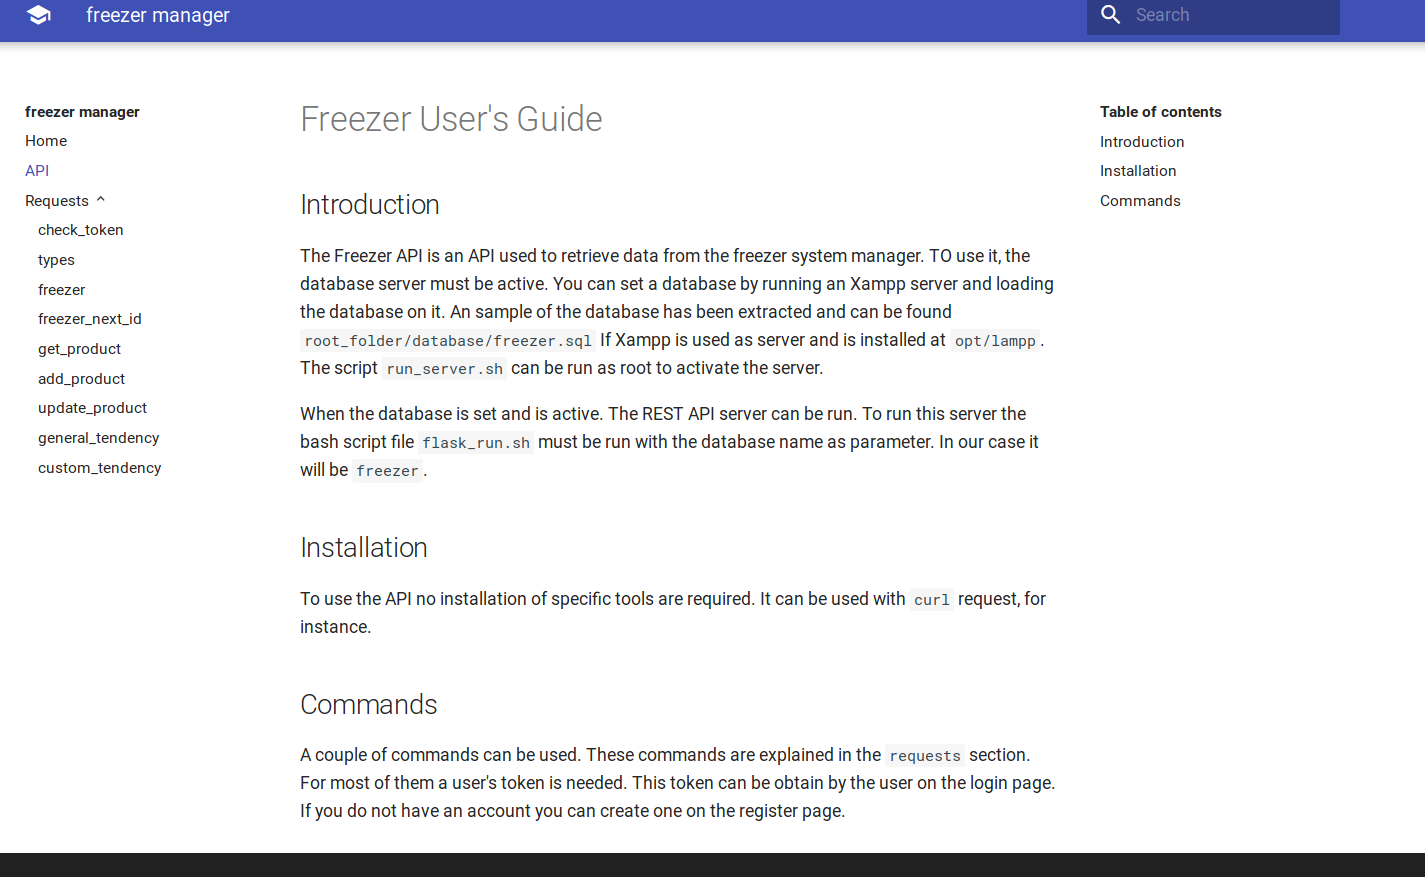
\includegraphics[scale=0.25]{./images/documentation.png}
\caption{Documentation website}
\label{fig:adminPanel}
\end{figure}

The documentation site can be found \textit{documentation/api-documentation/site/index.html}
\section{External website}
To demonstrate that the API can used by thirds applications. I developed a external application that only communicate with the REST API. The aim of this application is to provide to a user a user-friendly dashboard. To have access to the dashboard a user token is required and must be submit here.

%% Mettre une image

If the token given is valid, four tiles will be displayed. Each tile refer to a specific section (\textit{types of products, management of freezers, management of products, and trends}). The user has the possibility to display and hide each section. By default all sections are hidden. If the user want to display one section it just needs to click on the display button and click again to hide the section.

%% mettre image

%% plain d'images et expliquer les differentes sections
concernant la section produits parler de la detection des produits ayant depaasé la periode recommendée



The external website is developed with several languages \textit{css, html, javascript}. Moreover, some frameworks et tools are used. To have a responsive website, the containers of the bootstrap framework are used. Bootstrap is very well known in the website world. It is one of the famous framework used to built the skeleton of a website. Ta have dynamic tables I used a plug-in called tablesorter developed with jquery  % parler de fontawsome
and finally for the plot generation I use chart.js \\

The rest of the website is developed from scratch with pure javascript (no framework used). I used the pure javascript instead of framework like jquery because I did not see the real benefits of a specific framework. Moreover, there are a plethora of javascript frameworks and most of them require some practice before using it.\\



Ce veut être une application "externe" a l'API REST et à la DB. Peut etre vu comme une société externe utilisant un service

Le but de cettte application est d'avoir une sorte de dashboard
bcp de javascript pur
javascript pur
bootstrap utilisé
essayé de le rendre convivial et intuitif
tablesorter utilisé pour table interactive 
4 panel different qui peuvent être caché ou afiché
permet d'afficher en rouge dans les produits ceux qui ont dépassé la date limite

\section{unit tests}
To test the different functionalities implemented with the REST API, some unit tests have been done. The list of tests done is not exhaustive and can be extended. The units tests essentially cover the routes of the requests, the status code returned depending of the request done, the JSON objects sent, the content-type sent, and the methods implemented.\\

The tests done are defined in the test folder \textit{REST\_api/tests/tests.py}. They are based on the \textit{unittest} python module.
\section{problems faced}
I did not encounter big problems for this project. The most challenging parts are probably to constructs the different architectures. The database architecture takes sometime to finally reach the one used in the project. I also thank Mr. Hiard for the advice he gave me concerning my database architecture. Concerning the architecture of the REST API built with flask, it is not an easy work to find the proper architecture since there is no a unique template for building it, it will depend of the problem to solve. With flask you can build an API with different manners. The direction that I took seems to be coherent but for a largest application I think working with \textit{blueprints} decorators provided by flask can help because you can encompass routes that share the same pattern.\\

Concerning the external website the most challenging part is probably to work with javascript and the asynchronous behaviour brought by the AJAX requests. Moreover working with pure javascript can help to understand how it is working but you need to write extra code to achieve the same job as a framework.
\section{future work}
The future of this freezer manager system is probably to use an ORM to do the requests instead of using MysqlDB to allow an easier maintenance that could be done by people how do not know sql language. The reason for not having chosen this method directly is jusitified by the fact that mysqldb module gives me the possibility to use SQL language and it was a goal that I was looking for.\\

Another point is to migrate the system on the stable version of flask and mix it with gunicorn or uwsgi. It is also interesting to leave the localhost area and test the system on a real environment.\\

Another interesting point to develop in the future is to set a logger system that saves everything done on the server. In case of a Ddos attack or if a malicious people Who stole a user token and tries to destroy the data that the victim saved on its account. With the logger we can see where the requests come from.\\

An interesting thing, perhaps too optimistic, would be to put the project available for everyone and put the project as an open project where every one can contribute to the project and also to have feedback from others people.
\section{Conclusion}
